\chapter{Use cases}\label{ch:usecases}

\figref{fig:usecases} shows the use cases UML diagram.

\begin{figure}[htb]
	\centering
	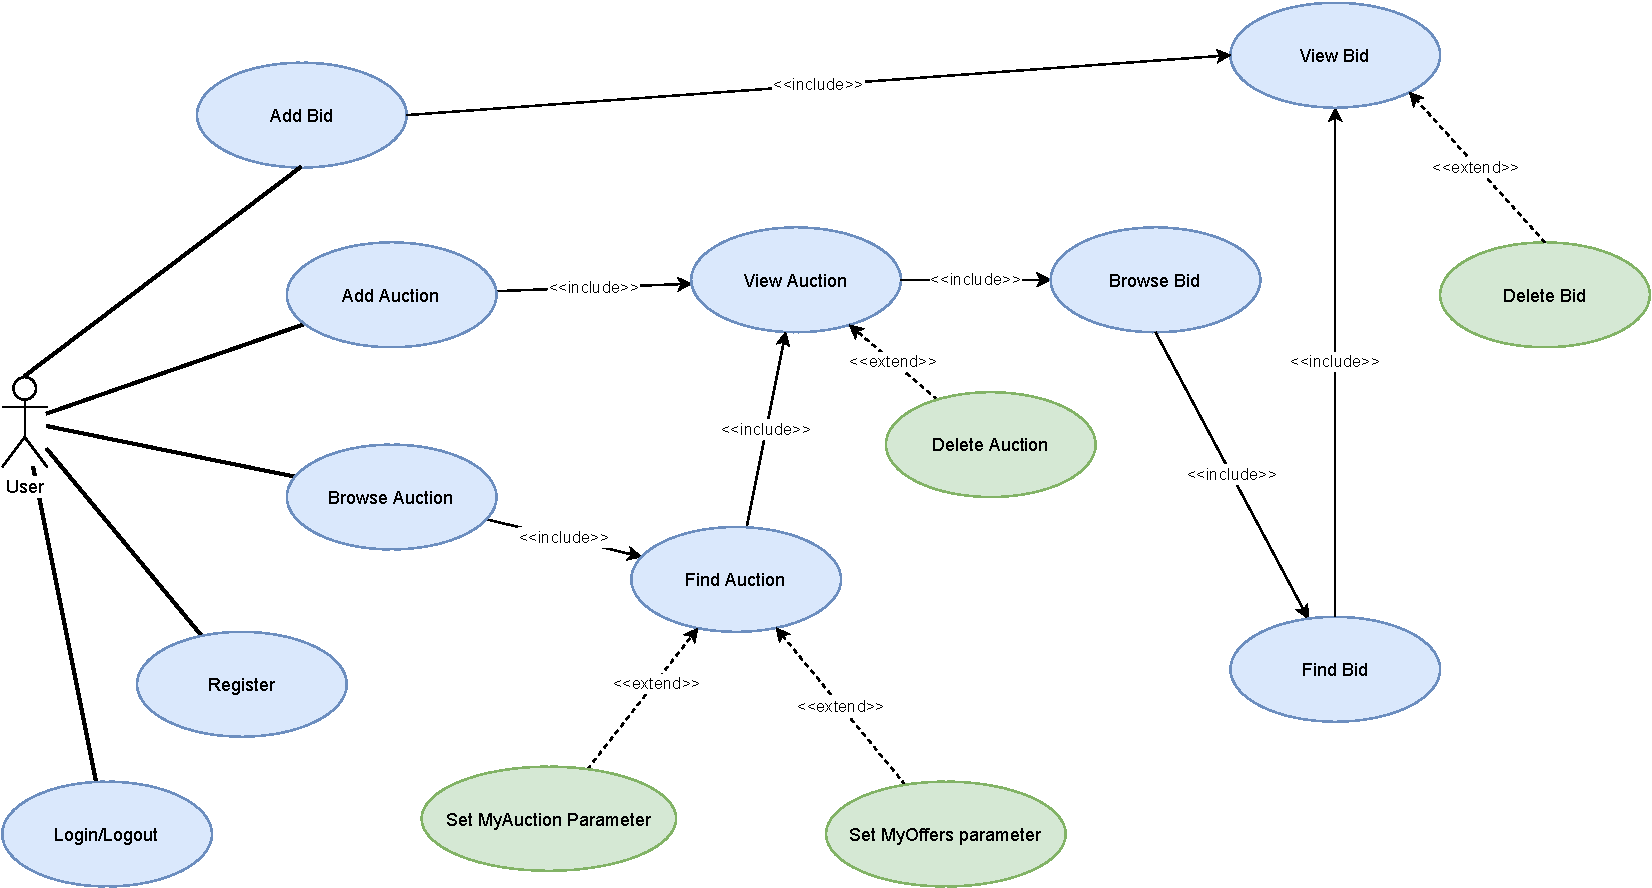
\includegraphics[width=\textwidth]{usecases}
	\caption{Use cases UML diagram}\label{fig:usecases}
\end{figure}

The following use cases are defined (all use cases, except Login and Register,
requires the user to be logged in):
\begin{description}
	\item[Login/Logout] A user can login in the application using its
		credentials (username, password). When logged in, he can logout
		from the application at any time.
	\item[Register] The first time a user uses the application he/she will
		be asked to register himself/herself, providing an username and
		a password.
	\item[Browse Auction] See the list of all available auctions saved in
		the application.
	\item[Find Auction] Search auctions selecting the auctions you have
		created (\code{MyAuctions} parameter) or selecting the auctions
		in which you have made a bid (\code{MyOffers} parameter).
	\item[View Auction] See all the information about an auction.
	\item[Add Auction] Add a new auction, providing name, image of the item
		to sell, description, the date of the end of the auction, the
		starting price for the auction, the minimum raise and the
		quantity of items that the user wants to sell.
	\item[Delete Auction] A user can delete an auction if it owns it.
	\item[Browse Bid] after an auction selection, a user can see all the
		bids he/she made for this auction.
	\item[Find Bid] Search a bid from the list.
	\item[View Bid] See all the information about a bid.
	\item[Add Bid] Add a new bid for an auction, providing the value of the
		bid and the quantity of items for which the bid is made.
	\item[Delete Bid] an user can remove a bid he/she made before.
\end{description}
